\documentclass[conference]{IEEEtran}
\usepackage{amsmath,amsfonts}
\usepackage{algorithmic}
\usepackage{algorithm}
\usepackage{array}
\usepackage[caption=false,font=normalsize,labelfont=sf,textfont=sf]{subfig}
\usepackage{textcomp}
\usepackage{stfloats}
\usepackage{url}
\usepackage{verbatim}
\usepackage{graphicx}
\usepackage{tabularx}
\usepackage{cite}
\hyphenation{op-tical net-works semi-conduc-tor IEEE-Xplore}
% updated with editorial comments 8/9/2021

\begin{document}

\graphicspath{{figures/}} %set folder for figures

\title{Speaker Recognition Using LGB Clustering on Mel Frequency Cepstrum Coefficients}

\author{
    Randall Fowler and Conor King
}

\maketitle

\begin{abstract}
    This paper presents a comprehensive study of a voice recognition system developed using Mel Frequency Cepstrum Coefficients (MFCC). The system design and methodology are explored in detail, with a focus on feature extraction and the use of MFCC. Performance is evaluated under various conditions, providing insights into its robustness and accuracy. While the system performs exceptionally well on homogeneous datasets, achieving 100\% accuracy, performance drops slightly on non-homogeneous datasets. For signal loss within certain frequency bands, the system retains reasonably well. In conclusion, the speaker recognition model has great performance with the small dataset provided and has areas for future improvements.
\end{abstract}

\begin{IEEEkeywords}
Speaker Recognition, Mel Frequency Cepstrum Coefficients, LGB Clustering, Feature Extraction
\end{IEEEkeywords}

\section{Introduction}
In the era of digital transformation, voice recognition has emerged as a pivotal technology, driving advancements in various sectors such as healthcare, automation, and security. This paper presents a comprehensive study of a voice recognition system developed using Mel Frequency Cepstrum Coefficients (MFCCs) and the LBG algorithm, a well-established method in the field of speech and audio processing \cite{lgb_paper}.

A detailed overview of the speaker classification processes used in this paper is provided as well as an explanation of the software environment. Selection of the hyperparameters is vital to the performance of the system, and an evaluation of different parameters is demonstrated. After a thorough testing of the system under various conditions was completed, a clear view of the strengths and weaknesses was summarized. With these insights, additional paths for further improvements are discussed.


\section{Methodology}
The central principle of voice recognition, and indeed of all classification, is feature extraction: determining or deciding which properties of the data are most discriminatory, i.e. contain the most information about the class of the data. For voice recognition, an initial approach might be to use the spectrogram of the sound; however, the features of the spectrogram are highly dependent on the specific words being spoken, the speed of articulation, and information about the timbre of the voice, while present, is still buried.

A more successful method is to use MFCCs. The training data is divided into frames of a given length with a given amount of overlap. These frames are windowed to mitigate the spectral distortion which would arise from abrupt changes at the beginning and end of the frame. Fourier Transform of each frame is taken, and the strength of the signal in several frequency bins is found. The exact number of bins used are critical in the efficacy of the overall recognition scheme. A popular principle is to use the Mel-frequency scale, which is designed to reflect how human aural acuity changes with frequency: it uses linear spacing below 1kHz and logarithmic spacing above.

Once the Mel-spectrum values are obtained for each frame, the logarithmic values are converted from one frequency domain to another frequency domain via the Discrete Cosine Transform (DCT). The result of transforming a frequency spectrum twice is known as cepstrum, and for this project, the cepstrum coefficients facilitate disentangling the vocal characteristics from the essential sound sequence.

After the MFCCs are found for each frame, these sampled values are best thought of as vectors in a n-dimensional space, where n is the number of mel-scaled bins used. A person’s voice will tend to produce vectors of a certain type, or types, corresponding to the qualities of their voice. These samples can then be plotted and analyzed via statistical methods. For this paper, the LBG clustering algorithm is used to group samples and compare group distances to other audio files \cite{lgb_paper}.

A centroid is defined as the mean of a grouping of MFCC samples. When the algorithm begins, it will start with a mean for the entire sample space, and then be split into two centroids. The new centroids will be placed equal distance apart in opposite directions. Samples will then be grouped to the nearest centroid, and the centroids will move toward the mean of the groupings. Centroids will continuously regroup with samples and move toward the mean until the movement is below a threshold. Then the two centroids are split, and the entire process repeats until a certain number of centroids is attained. When the algorithm finishes, the final centroids are saved as a codebook for that audio file.

A codebook is generated for each audio file in the training set. To classify any given audio file, it is split into frames and MFCCs are found for each frame. These MFCC vectors are then compared to each codebook by finding the distance from each sample to the nearest centroid. Whichever codebook has centroids with the smallest overall distance to the test MFCCs, this will be considered as the predicted label. The speaker whose audio file was used to train the predicted codebook label will be the predicted speaker.


\section{Design Decisions}
For the software design, a codebook class was created to hold the centroid locations. This class will handle the method of feature extraction, clustering algorithm, and saving of the centroid locations in memory. With the codebook class facilitating training of speaker models, a new set of data can then be compared to each of the codebook classes to get distance from centroids.

The class “codelibrary” behaves as an organizer of the codebooks; it has methods for creating and saving a set of codebooks corresponding to a set of training data in a given folder. Its prediction method finds the codebook which has the smallest distance from the given data. There is even a get accuracy method to run predictions on an entire folder of audio files and take the average prediction accuracy.

\subsection{Hyperparameter Selection}
The core system described in the Methodology section has several hyperparameters which can be tuned to improve performance on a specific instance of the speech recognition problem. These hyperparameters and their variable representations in our code, are described in table \ref{tab:hyperparameters}.

    \begin{table}
        \caption{Hyperparameter Selection}
        \label{tab:hyperparameters}
        \begin{tabularx}{\columnwidth}{|X|X|X|X|}
            \hline
            \textbf{Variable} & \textbf{Name} & \textbf{Description} & \textbf{Sweep Range}\\
            \hline
            $N$ & Frame Length & Number of samples in a frame & 1024, \\
            \hline
            $M$ & Hop Size & Number of samples between the start of every frame & $N$*(0.4, 0.5, 0.6)\\
            \hline
            window & Window Type & Type of window used for windowing the frames & Hamming, Hanning, Blackman, and Bartlett\\
            \hline
            $n\_mfcc$ & Number of MFCCs & Number of dimensions for each data point used for created the codebook & 20, 40, 60, 80\\
            \hline
            $size\_codebook$ & Size of Codebook & Number of centroids in the codebook & 16, 32, 64\\
            \hline
        \end{tabularx}
    \end{table}

    To improve the performance of our system on the in-class recordings, we performed a hyperparameter sweep over the values given in the Hyperparameter Range column of the table. Figure \ref{sweep_param_fig} contains an example of the results.

    \begin{figure*}[!h]
        \centering
        \subfloat[Hamming Window Accuracy for "Twelve"]{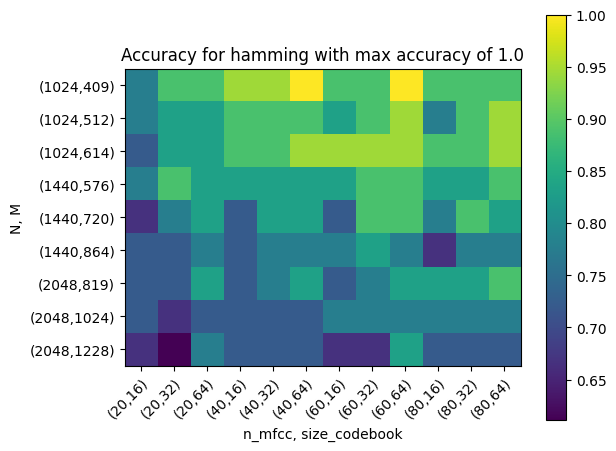
\includegraphics[width=0.3\textwidth]{twelve_sweep_hamming.png}}
        \hfill
        \subfloat[Hamming Window Accuracy for "Twelve"]{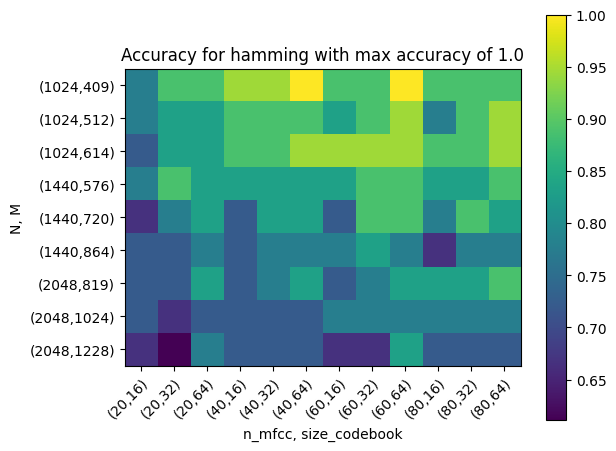
\includegraphics[width=0.3\textwidth]{twelve_sweep_hamming.png}}
        \hfill
        \subfloat[Hamming Window Accuracy for "Twelve"]{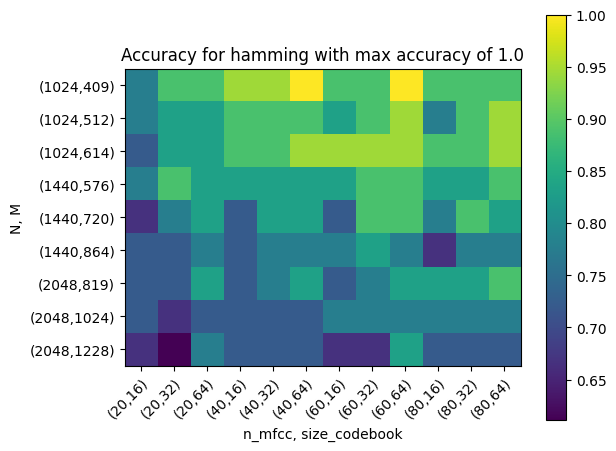
\includegraphics[width=0.3\textwidth]{twelve_sweep_hamming.png}}
        \hfill
        \subfloat[Hamming Window Accuracy for "Twelve"]{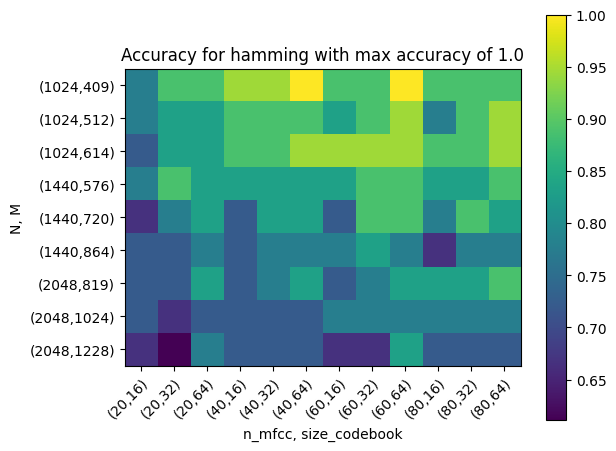
\includegraphics[width=0.3\textwidth]{twelve_sweep_hamming.png}}
        \hfill
        \subfloat[Hamming Window Accuracy for "Twelve"]{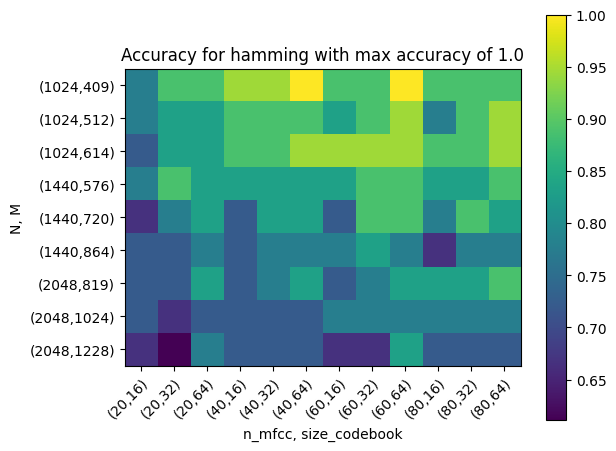
\includegraphics[width=0.3\textwidth]{twelve_sweep_hamming.png}}
        \hfill
        \subfloat[Hamming Window Accuracy for "Twelve"]{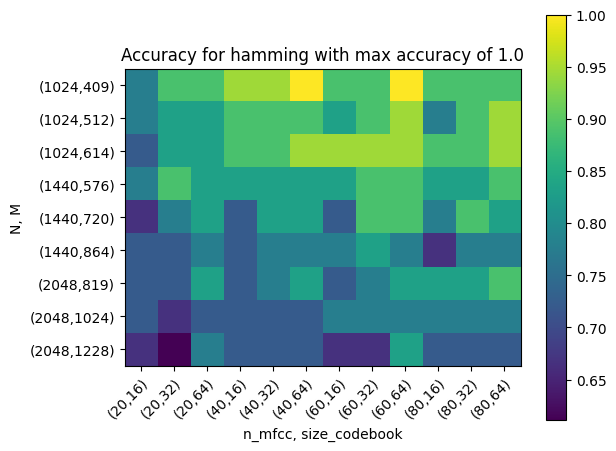
\includegraphics[width=0.3\textwidth]{twelve_sweep_hamming.png}}
        \caption{Hyperparameter Sweep Results}
        \label{sweep_param_fig}
    \end{figure*}

    For each window, the hyperparameters $N=1024$, $M=409$, $n\_mfcc$ = 40, and $size\_codebook = 64$ resulted in perfect accuracy, so those parameters were selected for the system. These hyperparameters were found for audio data recorded with a sampling rate of 48kHz, and alternative sampling rates would need to have updated $N$ and $M$ values.

\section{Experimental Tests}
    \subsection*{Test 1:}
    For the first test, human prediction on a given dataset was performed. The predictor familiarized themselves with the training data and gave an honest attempt at predicting the audio files. Only 3 out of 8 files were guess correctly with an accuracy of 0.375\%.

    \subsection*{Test 2:}
    The second tests was to visualize the waveform in time the time domain and as a periodogram. With the given data, the sampling rate was 12.5kHz and a plot of the waveform is in figure \ref{wave}. For 256 samples, this is equivalent to 20.5 ms. Spectrograms of this audio sample with different values of frame length ($N$) and overlap ($M$). The trade-off between time and frequency resolution as $N$ increases is clearly visible in figure \ref{stft}.

    \begin{figure}[!h]
        \centering
        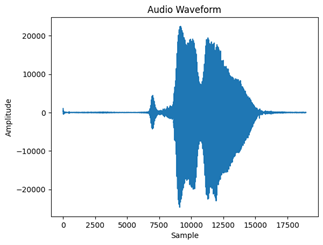
\includegraphics[width=0.5\textwidth]{audiowave.png}
        \caption{STFT with $N=256$ and $M=128$}
        \label{wave}
    \end{figure}

    \begin{figure*}
        \centering
        \subfloat[STFT with $N=128$ and $M=42$]{\includegraphics[width=0.3\textwidth]{stft1.png}}
        \hfill
        \subfloat[STFT with $N=256$ and $M=85$]{\includegraphics[width=0.3\textwidth]{stft2.png}}
        \hfill
        \subfloat[STFT with $N=512$ and $M=170$]{\includegraphics[width=0.3\textwidth]{stft3.png}}
        \caption{Spectrograms of Audio Sample}
        \label{stft}
    \end{figure*}

    \subsection*{Test 3:}
    The Mel-spaced filter bank responses in this system utilize a linear shifting of the weights to 100 Hz rather than the standard 1 kHz. After the spacing becomes logarithmic, the height of the triangles decreases to keep total energy in each filter constant, despite the increasing bandwidth. This Mel-spaced filter bank can be seen in figure \ref{weights}.

    \begin{figure*}
        \centering
        \label{weights}
        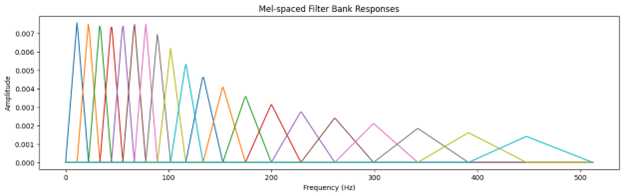
\includegraphics[width=1\textwidth]{melweights.png}
        \caption{Mel-Space Weights}
    \end{figure*}

    The Mel-frequency wrapping step allows a similar amount of information, from a classification standpoint, to be placed in each bin, leading to more efficient classification. Differences in the Mel-spectrum before and after wrapping can be seen in figure \ref{mel_spec}.

    \begin{figure*}
        \centering
        \subfloat[Mel-Spectrum before Wrapping]{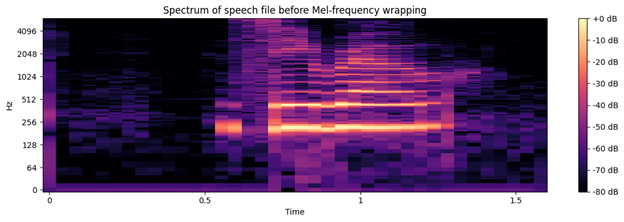
\includegraphics[width=1\textwidth]{melspectrum1.png}}
        \hfill
        \subfloat[Power of Mel-Spectrum]{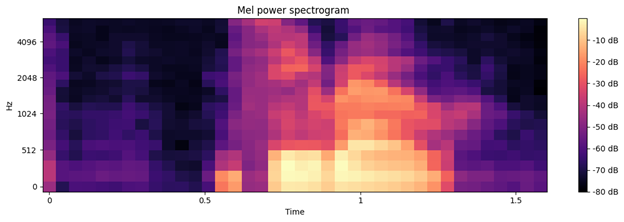
\includegraphics[width=1\textwidth]{melspectrum2.png}}
        \label{mel_spec}
        \caption{Mel-Spectrum of Audio Sample}
    \end{figure*}

    \subsection*{Test 4:}
    The feature extraction process is handled by the codebooks. The result of these codebooks are stored locally.

    \subsection*{Test 5 and 6:}
    Once MFCCs are collected from an audio file, these data points will be compared to centroid locations. Figure \ref{centroids} shows the centroids of the codebook for the given dataset along with the dataset's samples in two dimensions. In this case, there are 16 centroids, plotted along dimensions 0 and 1 out of the 40 MFCCs.

    \begin{figure}
        \centering
        \label{centroids}
        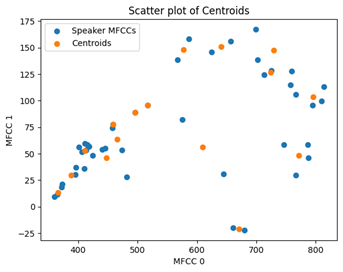
\includegraphics[width=0.5\textwidth]{centroids.png}
        \caption{Centroids of Codebook}
    \end{figure}

    \subsection*{Test 7:}
    This was the baseline test of the system on the provided training and test data. It creates a codelibrary based on the training data, and then tests the 8 test data files. The system had an accuracy of 100\% with the following hyperparameters: $N = 256$, $M = 100$, $n\_mfcc = 40$, window = Hamming, $size\_codebook = 64$.

    \subsection*{Test 8:}
    This test creates a notch filter at a given frequency and with a given quality factor, and then creates a new set of test files after applying the filter. The same library as Test 7 predicts these new files. The notch filter was applied to frequencies near 215 Hz, 440 Hz, 1000 Hz, and 6000 Hz. Figure \ref{notch} represents the notch filter at 215Hz, and table \ref{notch_table} shows the accuracy of the predictions.

    \begin{figure}
        \centering
        \label{notch}
        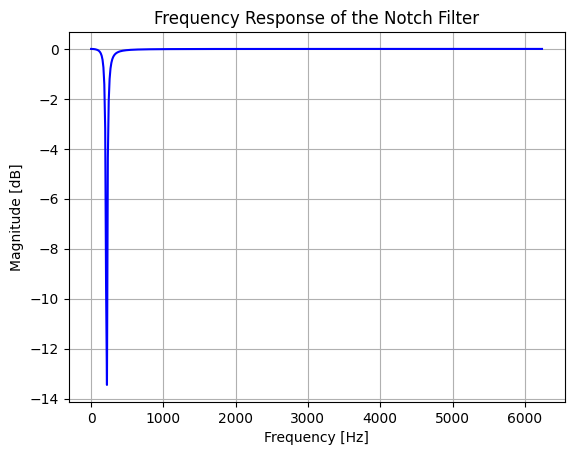
\includegraphics[width=0.5\textwidth]{notchfilter.png}
        \caption{Applied Notch Filter}
    \end{figure}

    \begin{table}[!h]
        \centering
        \caption{Accuracy of Notch Filtered Audio Files}
        \label{notch_table}
        \begin{tabular}{|c|c|}
            \hline
            \textbf{Notch Frequency} & \textbf{Accuracy} \\
            \hline
            215 Hz & 100\% \\
            \hline
            440 Hz & 100\% \\
            \hline
            1 kHz & 75\% \\
            \hline
            6 kHz & 87.5\% \\
            \hline
        \end{tabular}
    \end{table}

    The system appeared to be robust to losing certain frequency bands, although a notch filter at 1kHz was certainly detrimental. Within the 1 kHz range, key features within the human voice are lost, and the system is unable to predict the speaker with the same accuracy.

    

    \subsection*{Test 9:}
    To perform this test, new training and test datasets were created, composed of the original given datasets and 10 of the “zero” in-class recordings, chosen at random. Due to the different sampling rates, 12.5 kHz for the given and 48 kHz for the in-class recordings, the given data needed to be up sampled by a factor of 4. Hyperparameters remained as 1024 and 409 for $N$ and $M$ respectively since this was the optimal parameters in the last parameter sweep. A new code library was trained on the new training dataset and the accuracy on the testing audio files was 0.83.

    \subsection*{Test 10:}
    This test simply consisted of training and testing the system on the “twelve” in-class recordings. The accuracy of the system was found to be 100\%.

    A training and test dataset composed of every audio file, including an up sampled version of the given audio recordings, are used to train and test the system. The accuracy of the system was found to be 88.9\%.

    Finally, the system was tested on the ability to distinguish between the words “twelve” and “zero.” The accuracy of the system was found to be 100\%. This included incorrect predictions on the speaker, but the prediction of the word was correct.
    

\section{Conclusions}
Overall, the system was reliable at predicting homogenous datasets. For datasets which all had the same sampling rates and background noise characteristics, the system and hyperparameters selected achieved 100\% accuracy. When the data became non-homogeneous, in tests 9 and 10, performance suffered somewhat, although the accuracy remained above 80% in all cases. To improve this, a more precise rate-changing scheme might prove effective, as well as applying a filter to remove background noise. The system was robust to losing certain frequency bands, although a notch filter at 1kHz was certainly detrimental.
Other improvements which could be made are clipping the ends of the audio files, removing occasional loud background noise, and normalizing each audio file. Normalizing the energy for the audio files would reduce the influence on amplitude of the signal since loudness does not support classification.

\section*{Contributions}
Randall Fowler developed the tool set, software environment, to create codebooks and predict speakers, and sweep hyperparameter values. Conor King refined the software environment, tested implementation, and wrote the report.
\section*{Acknowledgment}
Thank you to Dr. Ding for the guidance and support for this class project.

\begin{thebibliography}{1}
    \bibliographystyle{IEEEtran}
    
    \bibitem{lgb_paper}
    Y. Linde, A. Buzo \& R. Gray, “An algorithm for vector quantizer design”, IEEE Transactions on Communications, Vol.
28, pp.84-95, 1980.
    
    
\end{thebibliography}

\end{document}


